\chapter[Extensive air showers and UHECR composition]{Extensive air showers}
\label{sec:showers}

In this chapter, we give an introduction to extensive air showers
(or only \emph{air showers}, for shortening).
Althought the physics behind these objects is very rich,
in this text we will give more focus on the selected topics
which are more relevant in the context of this thesis.
More detailed and extended materials about the topic can be found
in Refs.~\cite{GaisserBook,GriederBook}.

In~\cref{sec:showers:phen} we start by a phenomenological description
of the air shower development, focusing on the particle production in
both electromagnetic and hadronic component of te shower. 
In~\cref{sec:shower:simulations} we present the most relevant aspects
of air shower simulations, which are currently necessary to study
the  physics and to interpret the measurements of air showers.
Finally in~\cref{sec:shower:simulations} we present a compilation
of air shower measurements, focused on the range of high energy cosmic rays.
At this point we approach the currently inconsistency between measurements and
simulations of the muonic related observables, which is the main motivation
for this thesis.


%%%%%%%%%%%%%%%%%%%%%%%%%%%%%%%%%%%%
\section{Extensive air shower phenomenology}
\label{sec:showers:phen}

An air shower starts with the collision of the primary cosmic ray particle
with an atmospheric nucleus. After this first interaction, the secondary
particle produced also interact with the atmosphere producing more
particles and so on. This succession of interactions with particle production
creates the cascade of particles that forms the extensive air shower.
For the sake of clarity, the description of the cascade is tradionally
done by spliting it into different components: the \emph{electromagnetic},
the \emph{hadronic} and, eventually, the \emph{muonic component}. It is also traditional
to describe the air shower development in terms of its longitudinal and lateral profiles.
The former refers to the shower development along the direction of its axis
while the latter refers to the distribution of particles
in a plane perpendicular to the shower axis.


The first interaction can produce tens or hundreds of
secondary particles, which are nearly all hadrons
with only an insignificant contribution of photons and leptons.
Among the produced hadrons, the dominant contribution is by far from pions ($>60\%$),
followed by kaons and nucleons at similar proportions ($\sim 10\%$). Other
types of mesons and baryons together count tipically for less than 5\% of
the particles~\cite{Calcagni:2017tws}.
Besides that, a very small fraction of nuclei can be produced
by the fragmentation of the target atmosphereic nucleus or the primary (in case it is also a nucleus).
After the first interaction, the following air shower development is mostly driven
by the subsequent processes involving the secondary pions.
The three types of pions ($\pi^+$, $\pi^-$ and $\pi^0$)
are produced at similar proportions, which means that about 2/3 of them are charged and
1/3 is neutral. The charged ones will be responsible to create more
hadrons and eventually muons, while the neutral ones will decay into photons,
feding the electromagnetic component of the shower.
The latter case is firstly described in~\cref{sec:showers:phen:em}
and the former in~\cref{sec:showers:phen:had}. 

%%================================%%
\subsection[Electromagnetic component and the \xmax]{\boldmath Electromagnetic component and the \xmax}
\label{sec:showers:phen:em}


Neutral pions can decay via the electromagnetic interaction
into two photons ($\pi^0\rightarrow \gamma+\gamma$)
with a very short decay length ($c\tau_0=25$ nm). Since in the atmosphere this decay length
is much shorter than the interaction one, nearly all the neutral pions end up decaying into
photons. The high energy photons produced interact electromagnetically, being the dominant
process the pair production ($\gamma\rightarrow e^++e^-$).
The electrons\footnote{In this text the term \emph{electrons} actually refers to electrons and positrons} 
produced, in turn, also interact electromagnetically, mainly through bremstralung, which
produces more photons. The succession of these two electromagnetic processes
creates a self-sustainable cascade of photons and electrons
that forms the electromagnetic component of the extensive air shower.
Since more neutral pions are produced in hadronic interactions of secondary
particles with atmospheric nuclei (again in the 1/3 proportion wrt the charged pions),
the same chain of electromagnetic interactions takes place again
and new lower energy electromagnetic cascades are produced.
This means that the energy carried by the hadronic particles
is partially, but constinuously, trasfered to electromagnetic particles.
After a few generations of hadronic interactions ($\sim 6$), about 90\% of
the primary energy is carried by the electromagnetic component.


The length scale of the bremstralung interaction, responsible to produce photons out of
electrons, is given by the radiation lenght, $X_0$, that is the average distance needed
to electrons to lose all but $1/e$ of its energy. In the atmosphere $X_0\approx 37\text{g/cm}^2$.
On the other hand, the lenght scale of pair production is of the same order
of $X_0$, only slightly larger ($\approx 1.3 X_0$). Because of the short lenght scale
given by $X_0$, the electromagnetic shower develops very rapidly, which
implies a fast increase of the number of particles and a fast decrease of their
average energy. As lower the energies of the particles, more relevant are the energy losses
due to ionization. The critical energy in which the ionization losses
becomes equivalent to the bremstralung ones is $E_c = 85 \MeV$ in the
atmosphere. After the average energy of electrons becomes of the order of $E_c$,
the number of particles starts to decrease, which creates the peaked shape
of the longitudinal profile of the electromagnetic component.


In the left plot of~\cref{fig:shower:phen:prof}
we show the average longitudinal profile of the number
of photons ($N_\gamma$) and electrons ($N_e$) in air showers initiated by protons and iron nuclei.
It is also shown for comparison the longitudinal profile of the
deposited energy (\dEdX) in the atmosphere by all the charged particles.
Because the number of particles in the shower is dominated
by the electromagnetic component, one can see that the shape of the
\dEdX profiles is basically the same as the $N_e$ one.
The depth correspondent to the maximum of these both profiles is called
the shower maximum and it is symbolized by \xmax. In air shower
experiments, the \dEdX profile can be acessed by telescopes which
measure the fluorescence light emitted by the interaction of the air shower
with the atmosphere. The \xmax of the shower can then be determined
from the \dEdX profile.

%%%%%%%%%%%%%% LONG PROFILES %%%%%%%%%%%%%%%
\begin{figure}[!ht]
  \centering
  
  \begin{overpic}[clip, rviewport=0 0 1 1,width=0.45\textwidth]{electron_profile}
    \put(18,60){}
  \end{overpic}
  \begin{overpic}[clip, rviewport=0 0 1 1,width=0.45\textwidth]{muon_profile}
    \put(18,60){}
  \end{overpic}
  
  \caption{}
  \label{fig:shower:phen:prof}
\end{figure}

The dependences of \xmax with the primary energy ($E_0$) and with the nuclear
mass of the primary particle ($A$) can be expressed by the relation
\begin{equation}
  \langle\xmax\rangle = \lambda_\text{I}(A)+D_{10}\;\log_{10}\left(\frac{E_0}{A}\right),
  \label{eq:shower:xmax}
\end{equation}
where $\lambda_\text{I}$ is the mean free path of the first interaction.
The quantity $D_{10} = \text{d}\xmaxmean/\text{d} \log_{10}E_0$
is called \emph{elongation rate} and it does not depend on $E_0$ and $A$.
Although the~\cref{eq:shower:xmax} is derived by simplistic analitytic models~\cite{Matthews:2005sd},
it can be certified by using full Monte Carlo simulations that this relation is valid
in very good approximation.

On the left plot of~\cref{fig:shower:phen:xmax}
we show the \xmaxmean as a function of the primary energy
for a set of simulated air showers. The logaritmic energy dependence is clear,
as well as the separation between proton and iron initiated showers.
This dependence of \xmaxmean on the primary mass comes from both terms
on the right side of~\cref{eq:shower:xmax}. The $\lambda_\text{I}$ term
decreases with increasing $A$, because the interaction cross section
is larger for heavier nuclei. The second term, $\log_{10}\left(\frac{E_0}{A}\right)$,
is a manifestation of the so called \emph{superposition principle},
which says that an air shower initiated by a nuclei of mass $A$ of energy $E_0$
is actually equivalent to a superposition of $A$ showers
initiated by protons with primary energies $E_0/A$.
Since \xmax is a longitudinal quantity, it is not affected, on average,
by the superposition of shower and it turns out that the term $\log_{10}\left(\frac{E_0}{A}\right)$
is actually equivalent to only one proton shower with energy $E_0/A$.


%%%%%%%%%%%%%% XMAX MOMENTS %%%%%%%%%%%%%%%
\begin{figure}[!ht]
  \centering
  
  \begin{overpic}[clip, rviewport=0 0 1 1,width=0.45\textwidth]{electron_profile}
    \put(18,60){}
  \end{overpic}
  \begin{overpic}[clip, rviewport=0 0 1 1,width=0.45\textwidth]{muon_profile}
    \put(18,60){}
  \end{overpic}
  
  \caption{}
  \label{fig:shower:phen:xmax}
\end{figure}


The difference between \xmaxmean for
proton and iron initiated showers is $\sim 100 \text{g/cm}^2$, as can
be seen on the right plot of~\cref{fig:shower:phen:xmax}. It is also clear that the elongation rate
$D_{10}$ is nearly constant with energy and does not depend on the primary mass.
For using \xmax measurements to infer the primary composition of
cosmic rays, both the differences on \xmax for different primaries and
the constancy of $D_{10}$ are relevant features. By comparing the measured \xmaxmean
with simulation one can infer the average composition and by measuring
the $D_{10}$ one can verify if the composition is changing with energy or not. 


Besides the \xmaxmean, the fluctuations of \xmax also carry relevant information
about the primary cosmic rays. On the right plot of~\cref{fig:shower:phen:xmax}
we show the standard deviation of the \xmax distribution, \xmaxsig,
as a function of the primary energy for proton and iron initiated showers.
Concerning \xmaxsig, a consequence of the superposition principle
is that the fluctuations of the \xmax of showers initiated by nuclei
are smaller than the fluctuations of proton showers. It is also necessary
to take into account the smaller fluctuations on the depth of the first
interactions in nuclei showers. As a result,
we can see on the right plot of~\cref{fig:shower:phen:xmax}   
that the differences between \xmaxsig of proton and iron initiated showers is
about $\sigma^p[X_\text{max}]-\sigma^{Fe}[X_\text{max}] \approx 40 \text{g/cm}^2$.

The study of cosmic rays composition by using the \xmaxmean and \xmaxsig
is usually called \xmax moments analysis. The \xmax measurements
and their composition interpretation are approached in~\cref{sec:shower:observables:xmax}. 



%%================================%%
\subsection{Hadronic component and muon production}
\label{sec:showers:phen:had}

Unlike the neutral pions, the charged ones can only decay weakly,
with a much longer decay length ($c\tau_0=7.8$ m)
than the electromagnetic $\pi^0$ decay.  
At high energies, however, their interaction length
is much smaller than the decay one. This means that most
of the charged pions actually interact with atmospheric nuclei
producing more particles at similar proportions as the ones produced
in the first interaction. While the neutral pions produced
fed the electromagnetic shower, as explained above, the charged ones
can keep interacting and producing more hadrons. The hadrons
produced by this chain of hadronic interactions compose the
hadronic component of the shower.

As lower the energy of the charged pions, larger the probability
that they decay instead of interacting again. The dominant decay channel
for charged pions is into muons and neutrinos
($\pi^+\rightarrow\mu^+\nu_\mu$ and $\pi^-\rightarrow\nu^-+\bar{\nu}_\mu$)
and the critical energy in which the probability of decaying is
equivalent to interacting is 85 \GeV. These decays are responsible
to produce the great majority of the muons of an air shower.
The tipical number of interactions of charged pions before
decaying into muons is 4-8~\cite{Meurer:2005dt}. 

Apart from pion decays, a considerably fraction of the muons reaching
the ground is produced by the decay of charged kaons.
In~\cite{Meurer:2005dt,MeurerThesis} the muon
production in air showers was studyied in details and it was found
by using simulations that $\sim 90\%$ of the muons come from the decay
of charged pions and $\sim 10\%$ of charged kaons. While these particles
are called \emph{mother}, the particles which interacted hadronically
with an atmospheric nucleus to produce them are called \emph{grandmother}.
Thus, concerning the properties of the grandmother particles,
it was found that more than 70\% of them are pions, $\approx 20\%$ are nucleons
and $\approx 6\%$ are kaons. In~\cref{fig:shower:phen:ioana} the energy distributions of the
grandmother particles are shown and we can see the contribution from these
different types of particles~\cite{\IoanaICRC}.
The dominance of pions as gradmother particle is clear,
as well as the fact that most of the interactions of the grandmother particles
occur at energies of order of $\sim 100 \GeV$.

%%%%%%%%%%%%%% IOANA PLOT %%%%%%%%%%%%%%%

\begin{wrapfigure}{r}{0.5\textwidth}
  \centering
  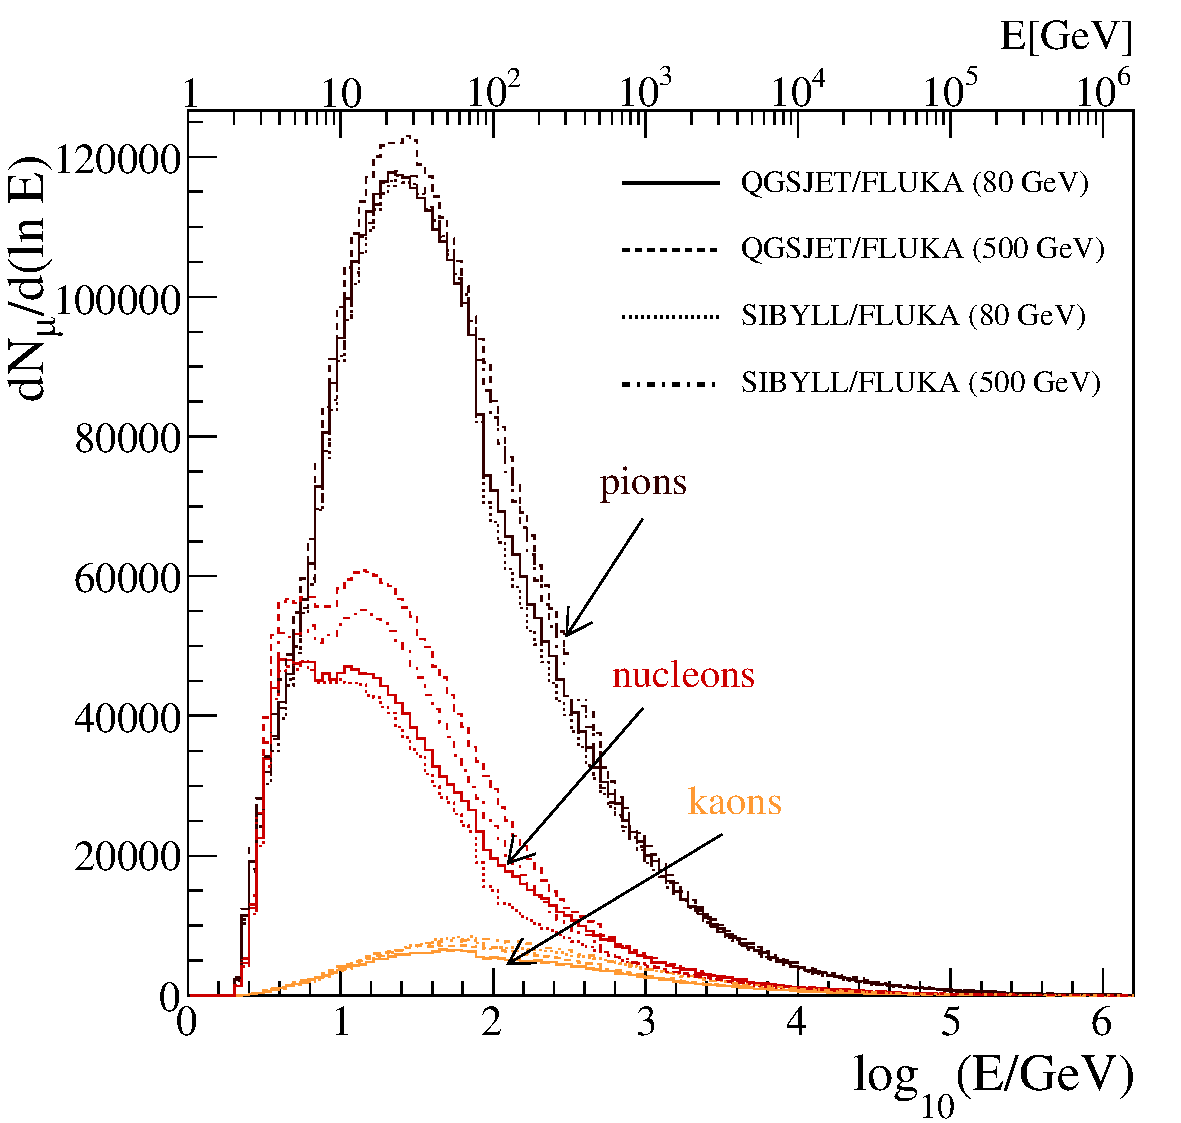
\includegraphics[width=0.5\textwidth]{energyDistAuger}
  \caption{\cite{\IoanaICRC}}
  \label{fig:shower:phen:ioana}
\end{wrapfigure}


%\begin{figure}[!ht]
%  \centering
%  \begin{overpic}[clip, rviewport=0 0 1 1,width=0.5\textwidth]{energyDistAuger}
%    \put(18,60){}
%  \end{overpic}
%  \caption{\cite{\IoanaICRC}}
%  \label{fig:shower:phen:ioana}
%\end{figure}


Although the interaction of the grandmother particle is very important,
it has to be noted that the whole chain of hadronic interactions, which are
mostly pion-air interactions, influence the muon production. This means
that any shower observable related to the muonic component is sensitive to the
properties of hadronic interactions which occur along the shower. The particle
production in these hadronic interactions is particularly important and,
in the context of this thesis, it is worthwhile to point out the effect of
(anti)baryon production. Most of the (anti)baryons produced are
nucleons (\proton, \antiproton, \neutron and \antineutron) and they
are all produced in similar proportions. Since these particles
can only interact again, their energy surely fed the
hadronic component, which means that it is partially converted
into muon production. Because of that, the increase of (anti)baryon
production in hadron-air interactions has been considered a very important
mechanism to increase the total number of muons in the shower~\cite{\EposPaper,Drescher:2007hc}.
Then, in view of the muon deficit problem, which is presented in~\cref{sec:shower:observables:nmu},
understanding the particle production in pion-air interactions turns to be
very important. Therefore, the~\cref{sec:hadron} of this thesis is dedicated to the measure of
the hadron production in pion-carbon interactions.

Besides increasing the number of muons, increasing the (anti)baryon
production in hadron-air interactions also affects the energy spectra
of the produced muons. It was argued in Ref.~\cite{\EposPaper} that
larger (anti)baryon production implies in shifting the muon energy spectra
to lower energies. Since acessing the energy spectra of muons at the ground
is very challenging experimentally, in~\cref{sec:observable} we propose
a new observable to be used for that considering experiments with
two different muon detectors.


On the left plot of~\cref{fig:shower:phen:prof}
we show the average longitudinal profile of
the number of muons, as well as the muon production,
for proton and iron initiated showers. First we can see that the
number of muons in iron initiated showers is substantially larger than
in proton showers. The reason for that is the fact that the first interaction
of a heavier primary produces a larger number of secondary hadrons, which
means that more hadronic sub-showers are generated and consequently
more muons are produced.
Second, we can see by comparing both plots of~\cref{fig:shower:phen:prof} 
that the muons are much weakly attenuated, after the shower reaches its maximum number of muons,
than the electrons. The number of muons after the maximum depth decreases very slowly
and after a certain atmospheric depth, only the muonic component survives to the attenuation.


The number of muons (\nmu) observed
at a given atmospheric depth is a tipical quantity of the shower.
A relation between \nmu and the primary energy ($E_0$) and mass ($A$)
can also be obtained from simplified analytic models~\cite{Matthews:2005sd}
and confirmed by full Monte Carlo simulations~\cite{AlvarezMuniz:2002ne}.
This relation is 
\begin{equation}
  \nmumean \approx A^{1-\beta} E_0^\beta,
  \label{eq:shower:nmu}
\end{equation}
where $\beta\approx 0.9$~\cite{AlvarezMuniz:2002ne}.
The energy and primary mass dependence
of \nmumean can be seen in~\cref{fig:shower:phen:nmu},
where we show the \nmumean as a function of energy,
again for proton and iron initiated showers.
Results of measurements of \nmu, as well as other
observables related to the muonic component will be presented
in~\cref{sec:shower:observables}.

%%%%%%%%%%%%%% NMU MOMENTS %%%%%%%%%%%%%%%
\begin{figure}[!ht]
  \centering
  
  \begin{overpic}[clip, rviewport=0 0 1 1,width=0.45\textwidth]{electron_profile}
    \put(18,60){}
  \end{overpic}
  \begin{overpic}[clip, rviewport=0 0 1 1,width=0.45\textwidth]{muon_profile}
    \put(18,60){}
  \end{overpic}
  
  \caption{}
  \label{fig:shower:phen:nmu}
\end{figure}


%%%%%%%%%%%%%%%%%%%%%%%%%%%%%%%%%%%%
\section{Air shower simulations}
\label{sec:shower:simulations}

In this section we give a short overview of the air shower simulations,
including a description of the most used simulation codes
in~\cref{sec:shower:simulations:codes} and
an overview of the hadronic interaction models used by them, in~\cref{sec:shower:simulations:models}. 
Besides the hadronic interaction models, the air shower simulation codes also
make use of electromagnetic interaction models. The commonly used one is \EGS~\cite{Nelson:1985ec}
Since the electromagnetic proccesses are properly described by quantum electrodynamics (QED),
their modelling is not considered to be a significant
source of uncertainties on the air shower simulations.
Because of that, we will only focus here on the hadronic interaction models,
which, in turn, are the most relevant source of uncertainties.
More detailed approaches to the topic can be found
in Refs.~\cite{Knapp:2002vs,Engel:2011zzb,Allen:2013ofa}.


%%================================%%
\subsection{Simulation strategies}
\label{sec:shower:simulations:codes}

To simulate an air shower taking into account all the
relevant aspects is surely a very complex task.
All the particles produced have to be propagated 3-dimensionally
thought the atmosphere and their interactions with atmospheric atoms
have to be properly modelled. The effect of the
structure of the atmosphere with changing density
and the earth magnetic field also have to be taken into account.
Besides that, the extremely large number of particles makes
the computational cost of an air shower simulation extremely large.
Because of that, the full simulation turns to be
impossible for pratical purposes and, thus, special strategies
have to be developed by simulation softwares to reduce the complexity
of the problem.


The most complete softwares apply Monte Carlo methods to simulate
the 3-dimensional propagation of the particles and their interactions
along the whole shower development.
This class of software includes \Mooca~\cite{\MoocaPaper},
\Aires~\cite{\AiresPaper} and \Corsika~\cite{\CorsikaPaper},
being the latter the one used in this thesis.
To reduce the computing time, an algorithm called \emph{thinning}
is usually applied~\cite{HillasThinning1,HillasThinning2}.
Intead of following all the particles, by using the
thinning algorithm only a number of them are selected
to be followed and a weight is given to these particles
which corresponds to the number of particles that
are not being followed anymore.


A few parameters is usually needed
to set up the thinning configuration. As an example, in \Corsika
the maximum particle energy in which the thinning algorithm is applied is
set by the $\varepsilon_\text{th}$ parameter, which is actually the fraction 
with relation to the energy of the primary. This parameter can be set separetely for
electromagnetic and hadronic particles and tipical values are between $10^{-2}--10^{-7}$.
As smaller the values of $\varepsilon_\text{th}$, more precise the simulation will be,
but with the cost of longer computing time. The maximum weight allowed is also a parameter to be set
and its tipical values lie between 100-10000. Since the thinning algorithm removes
the important information of the geometrical spread of the particles, for some analysis
an \emph{dethinning} algorithm has to be applied~\cite{Stokes:2011wf}.

A second class of simulation softwares, called \emph{hybrid}, makes use of Monte Carlo techniques
to simulate only the interactions at the highest energies and, below a certain
energy threshold, cascade equation are applied~\cite{Bossard:2000jh} to compute the
number of each type of particle as a function of the amospheric depth.
This means that the solution of the cascade equation gives only a 1-dimensional
description of the shower and all the information about the lateral distributions of
the particles is lost. Since for many applications only the longitudinal profile
of the shower is needed, this class of software turns to be very usefull.
The very short computing time required to solve the cascade equations
makes these softwares very fast. One of the most used code of this kind
is \Conex~\cite{\ConexPaper},
which is used in this thesis. The \Seneca code~\cite{\SenecaPaper}  
also makes use of cascade equations but includes a re-sampling
algorithm to recover the lateral particle distributions in the final stages
of the shower. It is worthwhile mentioning that the current
version of the \Corsika software can also simulate showers in the hybrid mode,
similar to \Conex or \Seneca.


%%================================%%
\subsection{Hadronic interaction models}
\label{sec:shower:simulations:models}

The models used to describe the hadronic interactions at high energies 
are by far the most relevant source of uncertainties on the prediction of
air shower observables by simulations. Although the strong interactions can be
sucesfully described by the \emph{quantum cromodynamics} theory (QCD),
we are still not able to compute the bulk of hadronic particle production processes. 

The hadronic interactions are described by first considering hadrons as constituted
by point-like particles called \emph{partons}. Then, the interactions between partons
are treated diferently depending on the transfer momentum: \emph{hard} and \emph{soft}
proccesses, in which there is a large and small momentum transfer, respectively.
While the properties of hard proccesses can be properly computed by means of
perturbative QCD, the soft ones require either lattice calculations
or phenomenological models to be described. Because of the long processing time
required by lattice calculations, the phenomenological approach
is applied by hadronic interaction models.

All the currently used hadronic models for high-energy interactions
are based on Gribov's Reggeon Field Theory~\cite{Gribov1968,Drescher:2000ha}, in which
parton-parton scattering is described by the exchaging of particles
called \emph{reggeons} and \emph{pomerons}. Another examples of commom features
of all models are the application of minijet and string fragmentations models.
An intrinsic feature of these phenomenological models is the large number of parameters
that cannot be determined theoretically, but they have to be tunned instead.
For that, a large number of accelerator measurements are used. The problem with this
strategy is that the accelerator measurements cover only a small fraction
of the energy range and particle production phase space that is relevant
for describing air showers. 

The problem with the model tunning can be split in three parts.
First, the highest energy collisions studied in accelerators
($\sqrt{s} = 13 \TeV$ reached by LHC) is still much lower
energy than the interaction of a high energy cosmic ray ($\sqrt{s}\approx 400$ for
a \E{20} primary proton). Second, there is a lack of measurements
of particle production at the forward region, which is the most relevant
to understand particle production in soft interaction and also
the most relevant for the air shower development. Finally,
there is a lack of accelerator data concerning some colliding systems
that are very important for air shower physics,
e.g. pion-air and kaon-air interactions.

As a consequence of the phenomenological nature of the models
in combination with the problems with accelerator data listed above,
the predictions of air shower simulations with different hadronic
interaction models turn to be discordant. Because of that,
it is a commom approach to compare the air shower measurements to
simulations with a number of different models and to treat
the differences between them as a systematic uncertainty
of theoretical nature.

For air shower studies, the most currently used models
for high energy interactions are
\QGSJetLong~\cite{\QGSJetPaper}, \EposLong~\cite{\EposPaper},
\EposLHCLong~\cite{\EposLHCPaper}, \SibyllLong~\cite{\SibyllPaper},
\SibyllNewLong~\cite{\NewSibyllPaper} and \DPMJetLong~\cite{\DPMJetPaper}.
Among these, \QGSJetLong, \EposLHCLong and \SibyllNewLong are updated
to take into account recent LHC data.  

Below a certain energy threshold ($\sim 100 \GeV$), the hadronic interactions
in air shower simulations are described by the so called \emph{low energy models}, which
are much simpler than the high energy ones. The particle production, for example,
is usually modelled by means of empirical parametrizations.
The most used low energy models are \Urqmd~\cite{\UrqmdPaper},
\Gheisha~\cite{Gheisha1985} and \Fluka~\cite{\FlukaPaper}.
A review of these models can be found in Ref.\cite{Heck:2004rq}.
The influence of the low energy models on the number of muons in air
showers have been shown in Ref.\cite{Maris:2009uc}.
We show in~\cref{sec:observable} that they are also relevant
for the spectrum of the muons at the ground.


%%%%%%%%%%%%%%%%%%%%%%%%%%%%%%%%%%%%
\section{Measurements of air shower observables}
\label{sec:shower:observables}

In this section, a compilation of measurements of air shower observables
is presented. The main focus is on the high energy cosmic rays range ($E>10^{17}$ eV).
We start in~\cref{sec:shower:observables:xmax}
by the \xmax measurements which are the most reliable
observable to be used to infer composition of cosmic rays.
In~\cref{sec:shower:observables:nmu}, measurements of the
\nmu are presented and the muon deficit problem
is introduced.
In~\cref{sec:shower:observables:further}
we briefly mention further observables recently measured.
A summary is finally presented in~\cref{sec:shower:observables:summary}. 


%%================================%%
\subsection{Shower maximum and cosmic ray composition}
\label{sec:shower:observables:xmax}

The \xmax (see~\cref{sec:showers:phen:em}) can be measured directly
by fluorescence telescopes, which can measure the energy deposited
by the air shower along the atmosphere. This technique was first sucesfully applied
by Fly's Eyes experiment~\cite{\FlysEyesPaper},
posteriorly followed by HiRes~\cite{\HiResPaper} and recently it
has been used by Telescope Array~\cite{\TAXmaxPaper} and
Pierre Auger Observatory~\cite{\AugerPaper,\AugerXmaxPRDPaper}.
Another technique commonly used in the past to measure the \xmax
are the non-imaging Cherenkov detectors. From the lateral profile
of the Cherenkov light measured in surface detectors, it is possible
to infer the longitudinal position of the shower maximum~\cite{Hillas:1982wz,Patterson:1983qj}.
This method was used by Tunka~\cite{\TunkaPaper,\TunkaXmaxPaper},
Yakutsk~\cite{\YakutskPaper,\YakutskXmaxPaper} and CASA-BLANCA~\cite{\CasaBlancaXmaxPaper}.
In~\cref{fig:shower:observables:xmax:all}
we show a compilation of \xmaxmean measurements from \E{15.0}
up to the highest energies and
in~\cref{fig:shower:observables:xmax:uhe} we show the most up to date
\xmax results of Pierre Auger Observatory~\cite{\AugerXmaxICRC2017Paper}
and Telescope Array~\cite{TAComp2017}.
The \xmaxsig is also shown togheter with the \xmaxmean.

%%%%%%%%%%%%%% XMAX ALL %%%%%%%%%%%%%%%
\begin{figure}[!ht]
  \centering
  
  \begin{overpic}[clip, rviewport=0 0 1 1,width=0.7\textwidth]{xmax_kampert}
    \put(18,60){}
  \end{overpic}

  \caption{\cite{Kampert:2012mx}}
  \label{fig:shower:observables:xmax:all}
\end{figure}

%%%%%%%%%%%%%% XMAX UHE %%%%%%%%%%%%%%%
\begin{figure}[!ht]
  \centering
  
  \begin{overpic}[clip, rviewport=0 0 1 1,width=0.8\textwidth]{xmax_auger_icrc}
    \put(18,60){}
  \end{overpic}
  
  \begin{overpic}[clip, rviewport=0 0 1 1,width=0.4\textwidth]{xmax_mean_ta}
    \put(18,60){}
  \end{overpic}
  \begin{overpic}[clip, rviewport=0 0 1 1,width=0.4\textwidth]{xmax_sig_ta}
    \put(18,60){}
  \end{overpic}

  \caption{\cite{TAComp2017} \cite{\AugerXmaxICRC2017Paper}}
  \label{fig:shower:observables:xmax:uhe}
\end{figure}


The colored curves in~\cref{fig:shower:observables:xmax:all}
show the \xmaxmean predictions from
Monte Carlo simulations. It is traditional to show the predictions for
the lightest primary expected, protons, and for the heaviest, iron nuclei.
By comparing the \xmax measurements with the Monte Carlo predictions,
one can obtain information about the average composition of the primary cosmic rays.
Besides the comparison of the \xmax moments,
the full \xmax distributions can be compared and the fractions of different
groups of primaries can be fitted. This procedure has been applied by Pierre Auger
Observatory in Ref.~\cite{Aab:2014aea}.

The composition interpretation of the \xmax measurements
is only possible because this observable is well described
by Monte Carlo simulations using hadronic interaction models.
From~\cref{fig:shower:observables:xmax:all},
we can first see that the measured \xmaxmean lies
always in between the predictions for protons and iron nuclei.
Furthermore, it is important the fact that
the Monte Carlo predictions with different hadronic interaction models
do not diverge substantially, which reduces the model depencencies
on the composition interpretations of the measurements.

Another importante feature of the \xmax analyses is
that the detector biases can be fully removed and the measured values
of the \xmaxmean and \xmaxsig can be directly compared to
the ones from shower simulations, without the requirement of simulating
the detection process. The Pierre Auger Observatory remove most of the
detector biases by using the so called \emph{fiducial volume cuts},
which reduces significantly the number of events~\cite{\AugerXmaxPRDPaper}.
On the other hand, because of the lack of statistics,
Telescope Array opt for not to perform any strategy to unbias the \xmax moments.
Intead, the measurements are compared to
simulation that include all the detector effects. As a consequence,
the \xmax moments as measured by both experiments cannot
be compared to each other directly.

From~\cref{fig:shower:observables:xmax:uhe}, the composition interpretation
of both Auger and Telescope Array \xmax data seem to be incompatible.
The Auger data shows a clear changing of the average composition from a very light
composition around \E{18.3} to an intermediate one around \E{19.5}. This trending is confirmed
by the fits of \xmax distributions shown in Ref.\cite{Aab:2014aea}.
The Telescope Array data, on the other hand, shows a constant composition
which is dominantly light, between proton and helium nuclei on average, from \E{18.2}
up to the highest energies. This apparent inconsistency has been studied
by a working group formed of members of both collaboration and the most recent
conclusion is that, taking into account the detector effects intrinsic of the Telescope Array
measurements and all the systematic uncertainties, the results of Telescope Array
are actually compatible with the composition infered from Auger data up to \E{19}~\cite{VitorICRC2017}.
Above this energy it was possible to take any conclusion
because of the lack of statistics of the Telescope Array measurements. 


%%================================%%
\subsection{Number of muons and the muon deficit problem}
\label{sec:shower:observables:nmu}

In this section we present measurements of both the number of muons (\nmu)
and the muon density ($\rho_\mu$) in air showers.
Measurements of \nmu or $\rho_\mu$ at ground can
be done with several different types of surface detector arrays.
However, the muon measurements are strongly affected by specific features
of each experimental setup and, therefore, it is not possible in general
to compare the measurements from different experiments. The experimental features
which affect the most the muon measurements are the muon energy threshold,
the lateral distance interval in which the muons are detected and the observation
level. 

To be able to detect muons isolately, the detectors are usually shielded so the
electromagnetic component is absorbed before reaching being detected. This can
be done either by placing a layer of a heavy material on the top of the detector
or by buring it few meters below the ground level. It turns out that low energetic muons
also end up being absorbed, and as a consequence, each experiment measures
muons above a different energy threshold and the \nmu is different.
The lateral distance range in which the muons are detected is also
a specific feature of each experiment that affects strongly the \nmu. Since
the experiments are always made of granular arrays, the distance between the detectors
usually determine in which lateral distance the \nmu is estimated. Lastly,
the observation level of the experiment affects the \nmu because of the atmospheric attenuation,
which affects much strongly the electromagnetic component, but it is still relevant for
muon detections.

Among the results of measurements of \nmu and $\rho_\mu$ in air shower experiments,
we have selected three to present here. The first one are the
measurements by HiRes/MIA experiments of the density of muons at the ground
in air showers initiated by cosmic rays of energy approaximately in the range
between \E{17} and \E{18}. The experimental setup consisted of a set of fluorescence
telescopes of the HiRes experiment~\cite{\HiResPaper} combined with a detector array of
MIA~\cite{\MIAPaper}. The surface detectors were formed by scintilator counters
buried about 3 m below the ground level, which implies in an energy threshold for muons
of aroud 850 \MeV. The density of muons at a lateral
distance of 600 m ($\rho_\mu(600)$) was reconstructed and compared to simulations.
On the left plot of~\cref{fig:shower:observables:nmu} we reproduce
the plot of $\rho_\mu(600)$ as a function of the primary energy as published
in Ref.~\cite{\HiResMIAMuonPaper}.
By comparing the measured muon density with predictions from Monte Carlo simulations,
it was found that the $\rho_\mu(600)$ in data was larger than the predictions for
the heaviest primaries expected, iron nuclei. This result was clearly inconsistent
in terms of composition and the conclusion that could be taken is that
the Monte Carlo simulations are deficient in muon production.
This was the first manifestation of what is usually called \emph{muon deficit problem},
in 1999.

%%%%%%%%%%%%%% NMU %%%%%%%%%%%%%%%
\begin{figure}[!ht]
  \centering
  
  \begin{overpic}[clip, rviewport=0 0 1 1,width=0.3\textwidth]{hires_mia_muons}
    \put(18,60){}
  \end{overpic}
  \begin{overpic}[clip, rviewport=0 -0.12 1 1,width=0.35\textwidth]{icetop_muons}
    \put(18,60){}
  \end{overpic}
  \begin{overpic}[clip, rviewport=0 -0.06 1 1,width=0.3\textwidth]{has_nmu}
    \put(18,60){}
  \end{overpic}
  
  \caption{}
  \label{fig:shower:observables:nmu}
\end{figure}

The second measurement to be presented was performed
by IceTop detector~\cite{\IceTopPaper}, part of the IceCube experiment~\cite{\IceCubePaper},
by using ice-Cherenkov surface detectors.
The primary energy range of these measurements goes from \E{15} to \E{17}
and the density of muons at 600 and 800 m from the shower axis was estimated
as muon content observable. On the midlle plot of~\cref{fig:shower:observables:nmu}
we reproduce the result from the Ref.~\cite{\IceTopMuonPaper}
which shows the $\rho_\mu$ as a function of energy compared to simulation predictions
by using the \SibyllNewLong as hadronic interaction model.
The muon deficit can be again seen at energies around \E{17}. Althought these are still
preliminary results, it is worthwhile to present it here because they show that
the muon deficit problem is still existing at relatively low energies (<\E{18}),
even by using modern hadronic interaction models like \SibyllNewLong.


The third and final measurement presented here is
the one performed by Pierre Auger Observatory~\cite{\AugerPaper}.
Even that its standard surface array
does not contain muon detectors, the number of muons can be measured by Auger
in highly inclined showers ($\theta > 60^\circ$). For this type of showers
the electromagnetic component is almost totally attenuated by the atmosphere
and the signal at the water-Cherenkov tanks is dominated by muons.
On the right plot of~\cref{fig:shower:observables:nmu} we show the
average \nmu as measured by Auger compared
to simulations as published in Ref.\cite{\AugerHASMuonPaper}.
The primary energy range here is above \E{18.6} and the muon deficit is clear
at the whole energy range. It is important to point out that both models
which are shown for comparison are recent versions, updated with LHC results.
In Ref.~\cite{\AugerTopDownPaper} another Pierre Auger result
that confirms the muon deficit at energies
around \E{19} can be found, in which showers with $\theta < 60^\circ$ 
were used.

In conclusion, the muon deficit problem is known for almost two decades
and at the moment it prevents us to do composition studies based on the
measurements of the \nmu in air showers. In~\cref{sec:interpretation}
we present a method to interpret the energy evolution of the moments
of the \nmu measurements in terms of cosmic rays
composition, taking into account the muon deficit problem.


%%================================%%
\subsection{Further measurements}
\label{sec:shower:observables:further}

In this section we briefly mention four further
measurements of air shower observables, the first one
made by KASCADE-Grande experiment~\cite{\KASCADEGrandePaper}
and the remaining three by the Pierre Auger Observatory.

The KASCADE-Grande experiment can measure both
number of charged particles and number of muons
in air showers with primary energy between
\E{16.0} and about \E{17.5}. In a recent analysis, the
KASCADE-Grande collaboration has studied the evolution
of the \nmu with the zenith angle of the shower by using
a parameter called muon attenuation length ($\Lambda_\mu$). 
Since the atmospheric attenuation of the muonic component
depends on the energy of muons, the parameter $\Lambda_\mu$ turns to
be sensitive to the muon energy spectra. Thus, by comparing the measurements
to Monte Carlo predictions it is possible to test muon production
properties of the hadronic interaction models. On the left plot of~\cref{fig:shower:observables:further1}
we reproduce the plot from Ref.~\cite{Apel:2017thr} that compares the measured value of 
$\Lambda_\mu$ with simulations and what can be seen is that none of
the currently used models can describe properly the muon attenuation.
The primary energy range of this analysis is similar to the one of IceTop shown
in the previous section.


The second measurement to be presented is the longitudinal depth
of the maximum of the muon production profile (\xmumax),
which can be measured by using the temporal structure of the
water-Cherenkov detectors of Pierre Auger Observatory
in highly inclined showers~\cite{\AugerMPDPaper}.
The main results is the energy evolution of \xmumaxmean that is show
on the right plot of~\cref{fig:shower:observables:further1}.
Althought the composition interpretation of these measurements
depends strongly on the hadronic interaction model, it can be seen that
for both \QGSJetLong and \EposLHCLong the infered composition would be
much heavier than the expected from the \xmaxmean measurements. The \EposLHCLong
case is even worst because it implies in a composition even heavier than iron nuclei.
In Refs.~\cite{Ostapchenko:2016bir,Pierog:2015ifw}
it has been shown that \xmumax is very sensitive to the properties of
the pion-air interactions and therefore its measurements
can be effectively used to contrain hadronic models.


The third and forth observables to be mentioned are related to the quantity called
risetime that is defined as the time difference between the water-Cherenkov detectors
reach 10 and 50\% of their total signal. This quantity is sensitive to both the
electromagnetic and muonic component of the shower.
In Ref.~\cite{\AugerAsymmetryPaper} an analysis of the azimutal asymmetry of the risetime
was published where a parameter called \emph{risetime asymmetry},
$\sec(\theta)_\text{max}$, was defined.
In a second analysis, published in Ref.\cite{\AugerDeltaPaper}, the so called
\emph{delta method} was applied in which the risetime dependence
on the lateral distance is used to define
a parameter called $\Delta_\text{s}$. 
In~\cref{fig:shower:observables:further2}
we show the main results of both analysis. 
The conclusions from both analysis are similar, being that the composition
extracted directly from $\sec(\theta)_\text{max}$ and $\Delta_\text{s}$
are not compatible with the one infered from \xmax measurements.
However, the inconsistency is not
as strong as in the case of \nmu and \xmumax. This intermediate behavior can
be understood by the fact that the risetime parameter is not sensitive to
only the muonic content of air showers, but instead, to a combination
of the electromagnetic and muonic components.
It was shown in Ref.\cite{\AugerDeltaPaper} that the $\Delta_\text{s}$
parameter can be calibrated by using the \xmax measurements and as a result
consistent composition inferences can be done.


%%%%%%%%%%%%%% FURTHER 1 %%%%%%%%%%%%%%%
\begin{figure}[!ht]
  \centering
  
  \begin{overpic}[clip, rviewport=0 0 1 1,width=0.48\textwidth]{kascade_attenuation}
    \put(18,60){}
  \end{overpic}
  \begin{overpic}[clip, rviewport=0 -0.1 1 1,width=0.48\textwidth]{mpd_auger}
    \put(18,60){}
  \end{overpic}
  
  \caption{}
  \label{fig:shower:observables:further1}
\end{figure}

%%%%%%%%%%%%%% FURTHER 1 %%%%%%%%%%%%%%%
\begin{figure}[!ht]
  \centering
  
  \begin{overpic}[clip, rviewport=0 -0.03 1 1,width=0.44\textwidth]{asymmetry_auger}
    \put(18,60){}
  \end{overpic}
  \begin{overpic}[clip, rviewport=0 0 1 1,width=0.48\textwidth]{delta_auger}
    \put(18,60){}
  \end{overpic}

  
  \caption{}
  \label{fig:shower:observables:further2}
\end{figure}


%%================================%%
\subsection{Summary}
\label{sec:shower:observables:summary}


In summary, YYY


